\chapter{Spin-Exchange Optical Pumping}
\label{chap2}

\section{Overview}

Spin-polarized noble gases have been widely used for various purposes. In JLAB, polarized $^{3}$He is used as target for electron-scattering experiments. This is because a $^{3}$He nucleus has a pair of protons with paired spins and a single neutron that contributes the most of the nuclear spin. In MRI, polarized $^{3}$He has seen uses such as detecting structural damage in the lungs.

There are generally two ways of polarizing $^{3}$He: Metastability-Exchange Optical Pumping (MEOP) and Spin-Exchange Optical Pumping (SEOP). Our group focuses on SEOP as MEOP polarizes gas at relatively low pressure, thus further compression is required to produce target cells.

In SEOP, alkali metal is polarized by circularly polarized laser that's tuned to the D1 transition of it. $^{3}$He obtains polarization from alkali metal through spin exchange process. With the combination of hybrid alkali mixtures (typically Rb and K) and spectrally narrowed lasers, more than 70\% polarizations have been produced.

\section{Optical pumping}

\subsection{Rb for SEOP}

In optical pumping, Rb is often the alkali metal that's optically pumped by circularly polarized laser light. The angular momentum of a polarized photon is transfered to the valence electron of Rb atom. In the case of hybrid mixture of Rb/K, Rb is still the alkali metal that's pumped by laser light directly while K serves as a more efficient medium to transfer the polarization from Rb to $^{3}$He compared to direct transfer from Rb to $^{3}$He. Rb is so widely used mainly for its low melting point, the relative ease of acquiring laser at the Rb D1 line wavelength and the clear seperation between D1 (794.7nm) and D2 line (780nm). 

The Rb melting point is at 39.5$^{\circ}$C, so it's easy to achieve enough Rb vapor without having to drive the oven temperature too high. In our lab, depending on if the cell contains pure Rb or Rb/K mixture, the oven temperature can be between 85$^{\circ}$C to as high as 255$^{\circ}$C. Perhaps the most used oven temperature for hybrid is 235$^{\circ}$C which has empirically been a good temperature to produce Rb/K mixture vapor, while 85$^{\circ}$C is enough for pure Rb.

\begin{figure}[H]
	
	\centering
	\resizebox{0.91\textwidth}{!}{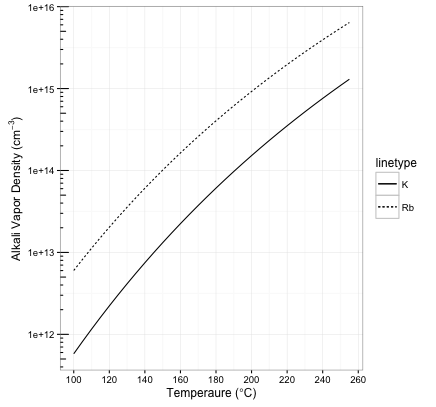
\includegraphics{AlkaliVaporDensity.png}}
	\caption[Rb And K Number Density Curves]{{\bf Rb And K Number Density Curves}}
	\label{fig:AlkaliVaporDensity}
	
\end{figure}

\subsection{Energy Levels of Alkali Metal in External Magnetic Field}

The Hamiltonian for ground state (L=0) alkali metal atoms in external magnetic field is:

\begin{equation}
{\bf H} = A{\bf I \cdot S} + g_{e} \mu_{B} S_{z}B_{z} + g_{N}{\mu_{N}}I_{z}B_{z}
\end{equation}

The first term $A{\bf I \cdot S}$ describes the coupling of the nuclear spin {\bf I} with the electron spin {\bf S} and is key to spin exchange, where A is the isotropic magnetic-dipole coupling coefficient. The resulting energy levels are referred to as hyperfine structure. The second and third terms describe the Zeeman splitting due to the presence of a weak external magnetic field. ${\mu}_{B} = 9.274 \times 10^{-24}J/T$ and ${\mu}_{N} = 5.051 \times 10^{-27}J/T$ are the bohr and nuclear magnetons. $g_{e}\approx2$ and $g_{N}\approx5.59$ are the electronic and nuclear Lande g-factors.

The linear relationship between energy levels and magnetic field only holds for weak magnetic fields as is the case with our lab where ~13 Gauss is used most of the time. When the Zeeman splitting grows relative to the hyperfine energy difference one would have to take into account the quantum mixing of the states, the result is described by Breit-Rabi Formula. With ~13 Gauss, the hyperfine term dominates the total Hamiltonian. The energy levels of $^{87}$Rb are shown in figure \ref{fig:Rb87EnergyLevels}.

\begin{figure}[H]
	\centering
	\resizebox{0.91\textwidth}{!}{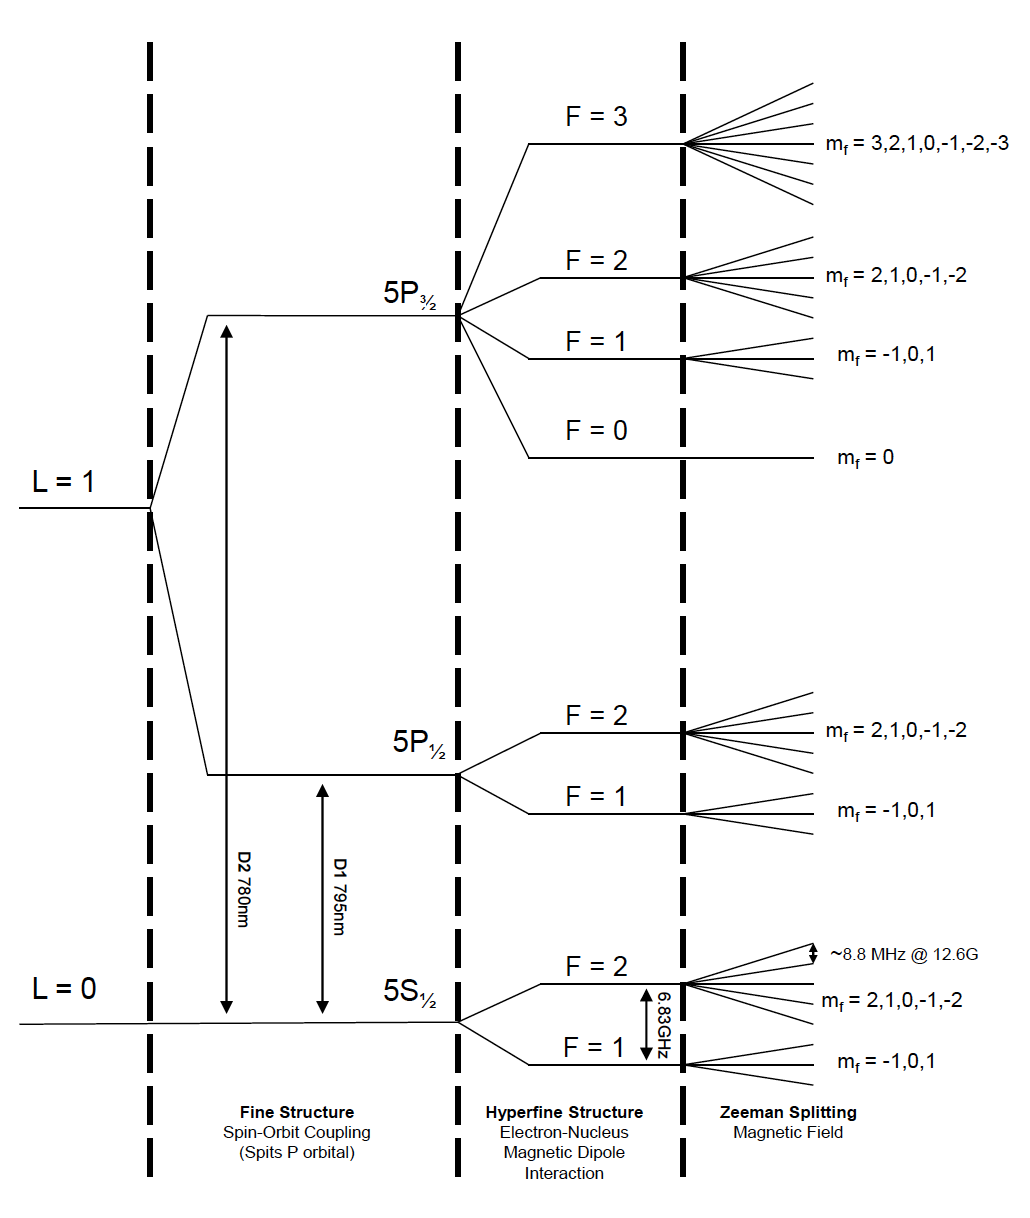
\includegraphics{Rb87EnergyLevelsPeter.png}}
	\caption{{\bf Level Diagram of $^{87}$Rb. The splittings are not to scale. Adapted from Dolph's PhD thesis.}}
	\label{fig:Rb87Energylevels}
\end{figure}

\subsection{Optical Pumping Process Overview}

For simplicity, the following discussion will ignore the nuclear spins for now. The inclusion of nuclear spins will increase the number of energy states but the optical pumping mechanism remains the same. In our typical setup, circularly polarized laser light is tuned to the D1 line of Rb and excites valence electrons of Rb from 5S$_{1/2}$ state to 5P$_{1/2}$ state as shown in figure \ref{fig:OpticalPumping} (2S$_{1/2}$ and 2P$_{1/2}$ states are used in the figure for the simple model described below). 

\begin{figure}[H]
	\centering
	\resizebox{0.91\textwidth}{!}{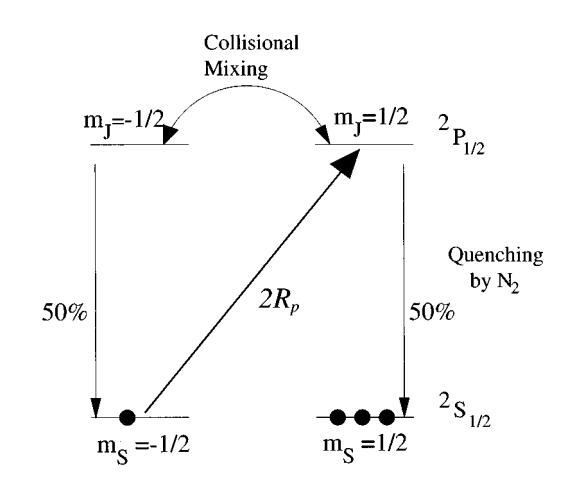
\includegraphics{OpticalPumping.png}}
	\caption{{\bf The interaction of alkali-metal atoms with left-circularly ($\sigma^{+}$) polarized light. (from Ref.\@ \cite{WalkerHapper})}}
	\label{fig:OpticalPumping}
\end{figure}

Although left-circularly polarized light is assumed in the figure, either circular polarization works the same. Conservation of angular momentum requires $\Delta$m = +1 as the figure show. Through collisions with other Rb atoms, excited electrons will be mix and evenly distribute on the two 2P$_{1/2}$ states. Electrons then decay to the two ground states with equal probabilities. The selection rule for the decay process is $\Delta$m = 0 or $\pm$1. Even though both grounds receive electrons from the decay, only the m = -1/2 state absorb the circular polarized photons, so atoms are in effect pumped to the m = +1/2 state. When we consider Rb with nuclear spins, both 5S$_{1/2}$ and 5P$_{1/2}$ states are split into more energy levels, but the net effect is still that the ground state with highest m accumulate atoms from those with lower m.

When the excited electrons decay back to the ground state, they emit unpolarized photons which can depolarize the gas. A small amount of N$_{2}$ gas is added into the cell (typically around 0.1 Amagats) to non-radiatively quench the excited electrons as N$_{2}$ molecules can absorb the released energy of spontaneous decays into their rotational and vibrational modes of oscillation. With an appropriate amount of N$_{2}$, the photon-emitting decays can be reduced to less than 5\%.

\subsection{Optical Pumping Rate}

The optical pumping rate at position $\vec{r}$ can be described by

\begin{equation}
R = \int \Phi(\nu, \vec{r})\sigma(\nu)d\nu
\end{equation}

where $\Phi(\nu,\vec{r})$ is the position dependent photon spectral flux density and $\sigma(\nu)$ is the photon absorption cross section. The cross section has a natural Lorentzian lineshape which is broadened by Doppler effect and pressure broadening. The pressure broadening effect dominates the lineshape as our cells normally have densities well above one amagat. $\sigma(\nu)$ follows the sum rule:

\begin{equation}
\int\sigma(\nu)d\nu=\pi r_{0}cf
\end{equation}

where $r_{0}=2.82 \times 10^{-13}$ cm is the classical electron radius and f=0.337is the transition oscillator strength. Thus the photon absorption cross section can be described by Lorentzian lineshape:

\begin{equation}
\sigma(\nu)=fr_{e}c\frac{\frac{\Gamma_{A}}{2}}{(\nu-\nu_{0})^{2}+(\frac{\Gamma_{A}}{2})^{2}}
\end{equation}

where $\Gamma_{A}$ is the pressure dependent FWHM. At the front of the cell, the photon spectral flux density is the product of a Gaussian spatial distribution and a Gaussian spectrum.

\begin{subequations}
	\begin{gather}
	\phi(\nu,\vec{r})=\phi_{0}(\vec{r})G(\nu) \\
	\phi_{0}(\vec{r})=\frac{P}{h\nu}\frac{2}{\omega^{2}\pi}e^{2r^{2}/\omega^{2}}\\
	G(\nu)=\frac{1}{\sqrt{2\pi}\sigma_{l}}e^{-(\nu-\nu_{l})^2/2\sigma_{l}^{2}}
	\end{gather}
\end{subequations}

where P is the laser power; $\omega$ is the beam waist;  $\sigma_{l}$ is the Gaussian width of the laser and $\nu_{l}$ is the central laser frequency.

\begin{figure}[t!]
	\centering
	\resizebox{0.91\textwidth}{!}{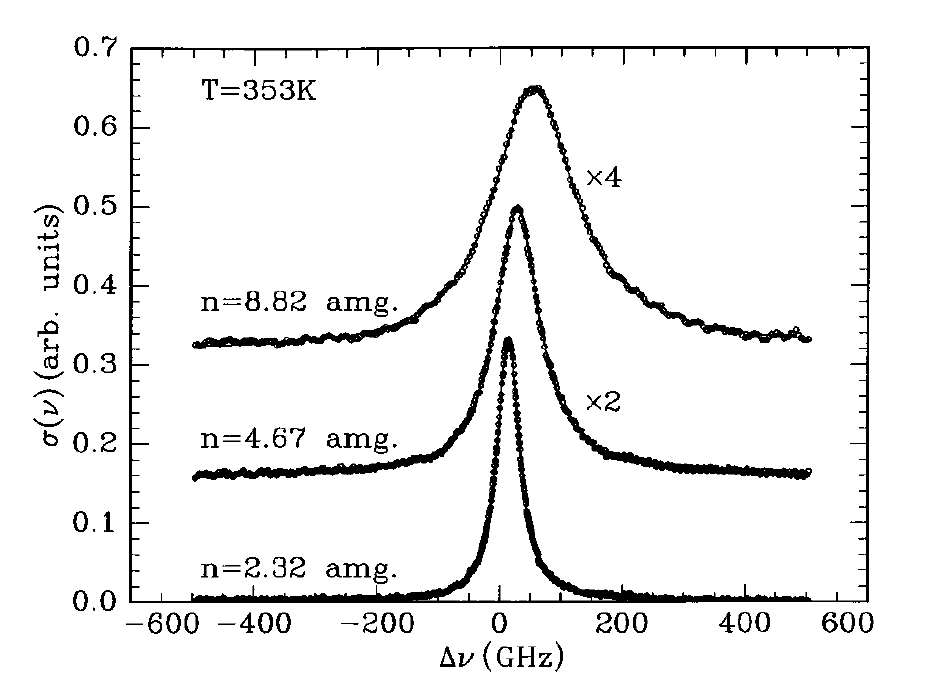
\includegraphics{AbsorptionLine.png}}
	\caption{{\bf Absorption cross section for Rb $D_{1}$ line in the presence of three different densities of $^{3}$He. (from Ref.\@ \cite{Romalis1997})}}
	\label{AbsorptionLine}
\end{figure}

\begin{figure}[t!]
	\centering
	\resizebox{0.91\textwidth}{!}{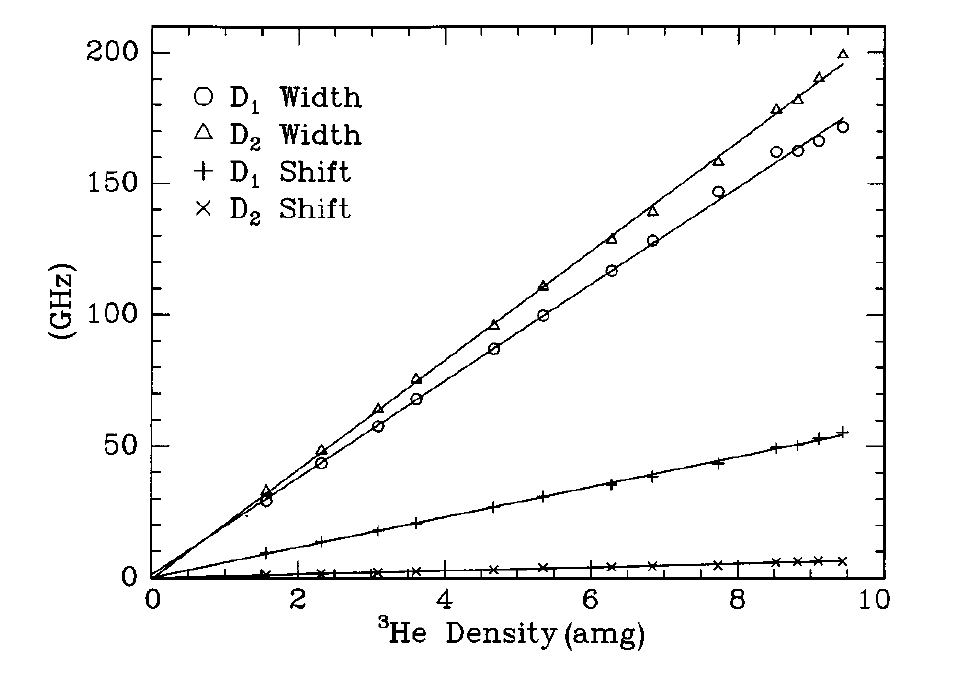
\includegraphics{PressureBroadening.png}}
	\caption{{\bf The shift and the broadening due to presence of $^{3}He$ for Rb $D_{1}$ and $D_{2}$ lines. (from Ref.\@ \cite{Romalis1997})}}
	\label{AbsorptionLine}
\end{figure}

\subsection{Polarization Time Evolution}

Although polarizations of Rb electrons are more complex, $^{3}He$ nuclei have an intrinsic nuclear spin of 1/2, and it's simpler to explain the math with spin of 1/2, let's define the polarization as the asymetry between +1/2 state and -1/2 state:

\begin{equation}
P=\frac{\rho_{+1/2}-\rho_{-1/2}}{\rho_{+1/2}+\rho_{-1/2}}=\rho_{+1/2}-\rho_{-1/2}
\end{equation}

where $\rho_{\pm 1/2}$ is the population in the $\pm1/2$ state.

The time evolution of polarization for both Rb electrons and $^{3}He$ follows the equation:

\begin{equation}
\frac{dP}{dt}=\gamma(1-P)-\Gamma \cdot P
\end{equation}

$\gamma$ is the polarization rate and $\Gamma$ is the depolarization rate in the above differential equation. The solution has the simple form of:

\begin{equation}
P(t)=Ce^{-(\gamma+\Gamma)t} + \frac{\gamma}{\gamma+\Gamma}
\end{equation}

Note the depolarization rate also contributes to the speed at which P approaches saturation. The saturated polarization is defined as the value of P in the limit t $\rightarrow \infty$:

\begin{equation}
P_{\infty}=\frac{\gamma}{\gamma+\Gamma}
\end{equation}

The initial polarization is defined as the value of P at t = 0:

\begin{equation}
P_{0}=C+\frac{\gamma}{\gamma+\Gamma}=C+P_{\infty}
\end{equation}

Thus, P(t) can be expressed as:

\begin{equation}
P(t)=(P_{0}-P_{\infty})e^{-(\gamma+\Gamma)t}+P_{\infty}
\end{equation}

In the case of polarizing Rb with a pump laser. $\gamma$ is the pumping rate R and $\Gamma$ is the Rb spin relaxation rate $\Gamma_{Rb}$. There is typically a small angle $\theta$ between the pump laser and the magnetic field that separates the different spin states of Rb valence electrons even though great effort has been made to minimize the angle. Thus P(t) can be rewritten as:

\begin{equation}\label{Pt}
P(t) = P_{0}e^{-(R+\Gamma_{Rb})t} + P_{laser}cos\theta \frac{R}{R+\Gamma_{Rb}}(1-e^{-(R+\Gamma_{Rb})t})
\end{equation}

$P_{laser}$ is the circular polarization of the pump laser which is above 99.5\%. Rb close to the front side of the cell can reach above 97\% (depends on the laser power and other factors) on the order of 100's of microseconds. As the laser propagates through the cell, power is attenuated by Rb vapor. Therefore Rb polarization at the back side of the cell is lower than that at the front side. One way to overcome the problem is to shine pump laser from both sides of the side which would lead to higher overall Rb polarization and $^{3}$He polarization.

Spins are thermally polarized with the presence of a magnetic field even without external pumping source. The probability for a spin to be in state s is:

\begin{equation}
Prob. = \frac{e^{-E_{s}/k_{B}T}}{\sum_{si}e^{-E_{si}/k_{B}T}}
\end{equation}

where $E_{s}$ is the energy of the state, $k_{B}$ is the Boltzmann constant and T is the temperature. Using the thermal distribution, under typical operating conditions, $^{3}He$ polarization is ~$10^{-9}$ and Rb polarization is ~$10^{-5}$. Both are negligible without active pumping.

\subsection{Rb Spin Destruction Rate}

There are two main mechanisms of Rb depolarization: the binary collisions with Rb, $^{3}$He and $N_{2}$ and the formation and breakup of van der Waals molecules, while the second mechanism is negligible for $^{3}$He cells. The Rb spin destruction rate can then be expressed as

\begin{equation}
\Gamma_{Rb}=k_{Rb-Rb}[Rb]+k_{Rb-^{3}He}[^{3}He]+k_{Rb-N_{2}}[N_{2}]
\end{equation}

where $k_{Rb-X}$ is the spin destruction rate constant and [X] is the density of X. Dolph has summarized these constants based on measurements from various groups:

\begin{subequations}
	\begin{gather}
	k_{Rb-^{3}He}(T)=55.9(9)\left(\frac{T}{473.15K}\right)^{3.31(12)}Hz/amg\\
	k_{Rb-N_{2}}(T)=290(30)\left(\frac{T}{473.15K}\right)^{2.0(25)}Hz/amg\\
	k_{Rb-Rb}=4.813(48)\times 10^{-13}Hz\cdot cm^{3}
	\end{gather}
\end{subequations}

For a pure Rb cell at 170$^{\circ}$C with the following densities in the pumping chamber:

\begin{subequations}
	\begin{gather}
	[^{3}He] \approx 8.0 amg\\
	[N_{2}] \approx 0.08 amg\\
	[Rb] \approx 6.0 \times 10^{14} cm^{-3}
	\end{gather}
\end{subequations}

The approximate spin destruction rates due to various gases are:

\begin{subequations}
	\begin{gather}
	\Gamma_{Rb-^{3}He} \approx 360Hz\\
	\Gamma_{Rb-N_{2}} \approx 20Hz\\
	\Gamma_{Rb-Rb} \approx 289Hz
	\end{gather}
\end{subequations}

The total spin destruction rate is 669 Hz.

\section{Spin Exchange}

Following equation \ref{Pt}, the time evolution of $^{3}He$ polarization can be expressed as:

\begin{equation}
P_{^{3}He}(t) = P_{0}e^{-(\gamma_{se}+\Gamma)t} + P_{Rb} \frac{\gamma_{se}}{\gamma_{se}+\Gamma}(1-e^{-(\gamma_{se}+\Gamma)t})
\end{equation}

The saturation polarization is 

\begin{equation}
P_{\infty} = P_{Rb}\frac{\gamma_{se}}{\gamma_{se}+\Gamma}
\end{equation}

where $\gamma_{se}$ is the spin exchange rate between $^{3}$He and Rb, and $\Gamma$ is the spin relaxation rate. 

\subsection{Spin-Dependent Interactions}

The key process in spin-exchange optical pumping is collisional transfer of polarization between optically pumped alkali-metal atoms and the nuclei of the noble gas atoms. As in Fig. \ref{SpinExchange}, the transfer of angular momentum occurs either while the atoms are bound in van der Waals molecules or in simple binary collisions. For $^{3}He$, binary collisions dominate, and the contribution from van der Waals molecules is negligible. The time scale for binary collisions is on the order of $~10^{-12}$ sec, so the collision can induce both $\Delta F=\pm1$ and $\Delta F=0$ transitions between hyperfine sublevels. For heavier noble gases like $^{129}$Xe at pressure of a few tens of Torr, the contributions of van der Waals molecuels can greatly exceed that of binary collisions. At several atms which is the typical operating pressure for SEOP, the time scale of van der Waals molecules is greatly limited by collision so that the binary collisions dominate.

\begin{figure}[t!]
	\centering
	\resizebox{0.91\textwidth}{!}{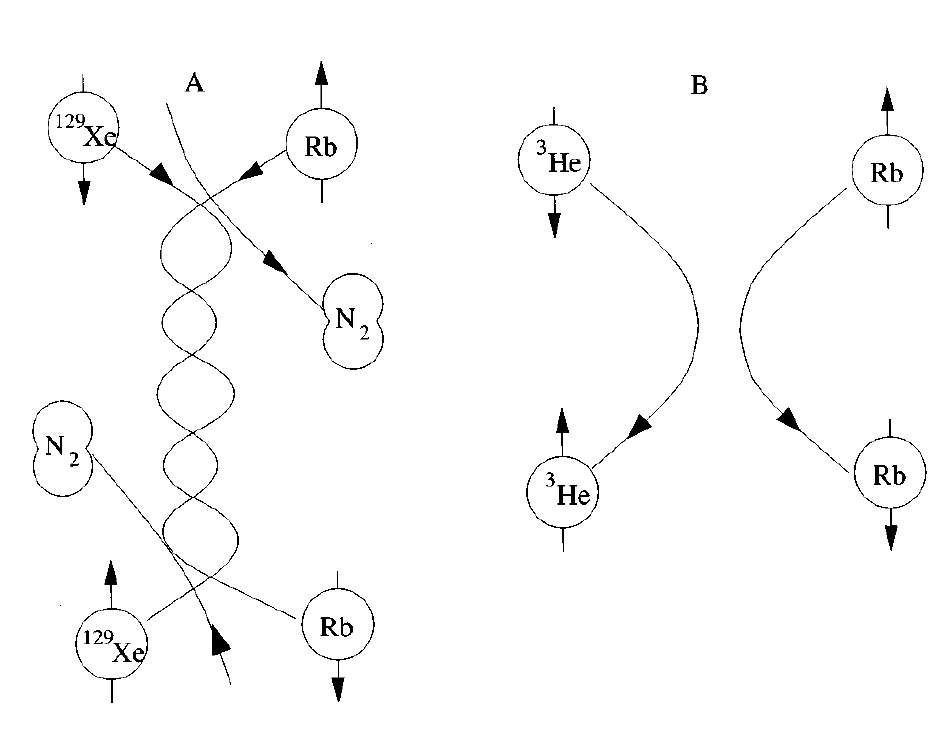
\includegraphics{SpinExchange.png}}
	\caption{{\bf A. Formation and breakup of alkali-metal/noble-gas van der Waals molecule. B. Binary collision between an alkali-metal atom and a noble-gas atom. (from Ref.\@ \cite{WalkerHapper})}}
	\label{SpinExchange}
\end{figure}

Spin-dependent interactions produce the spin transfer and relaxation. For SEOP, spin-rotation interaction between $\vec{S}$ and the rotational angular momentum $\vec{N}$ and the isotropic hyperfine interaction between $\vec{S}$ and the noble-gas nuclear spin $\vec{I}$ dominate the spin-exchange process:

\begin{equation}\label{V1}
V_{1}(\vec{R})=\gamma(R)\vec{N}\cdot \vec{S}+A(R)\vec{I}\cdot \vec{S}
\end{equation}

$\vec{I}_{a}$ and $\vec{I}_{b}$ are the nuclear spins of the atomic pair.

The spin-rotation interaction is caused by the magnetic fields from relative motion of the charges of the colliding atoms, and the isotropic hyperfine interaction comes from the magnetic field inside the nucleus of the noble-gas atom. 

An alkali-metal atom and a noble-gas atom interact via both a large spin-independent interaction $V_{0}(R)$ and a small spin-dependent interaction $V_{1}(R)$. At the high operating temperatures, $V_{0}$ determines classical collision trajectories, while $V_{1}$ acts as a small perturbation. We'll focus on $V_{1}$ below since it is responsible for spin exchange.

Including a few more terms that were neglected in Eq. \ref{V1}, the spin-dependent interaction $V_{1}(R)$ can be expressed as:

\begin{equation}
\begin{split}
V_{1}(\vec{R})=\gamma(R)\vec{N}\cdot \vec{S}+\sum_{k}A_{k}(R)\vec{I}_{k}\cdot \vec{S}\\
+\sum_{k}B_{k}(R)\vec{I}_{k}\cdot (3\vec{R}\vec{R}-1)\cdot \vec{S}\\
+\sum_{k}C_{k}(R)\vec{I}_{k}\cdot (3\vec{R}\vec{R}-1)\cdot \vec{I}_{k}
\end{split}
\end{equation}

\begin{figure}[H]
	\centering
	\resizebox{0.91\textwidth}{!}{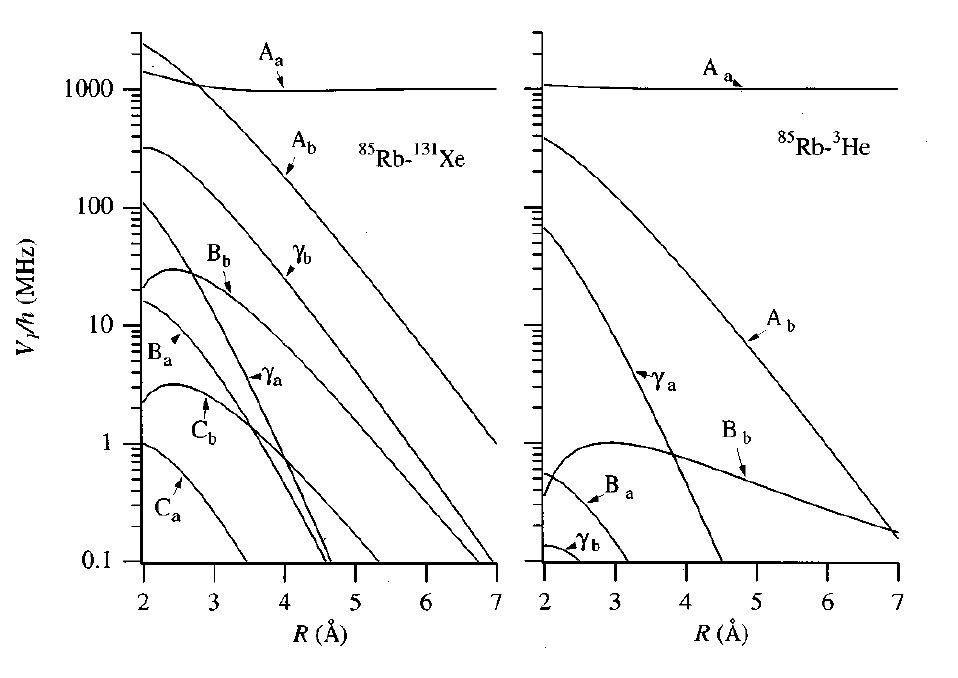
\includegraphics{V1.png}}
	\caption{{\bf Strengths of various spin-dependent interactions as functions of separation(from Ref.\@ \cite{WalkerHapper})}}
	\label{SpinExchange}
\end{figure}

where $\gamma$ is the coefficient of the spin-rotation interaction, while $A_{k}$, $B_{k}$, $C_{k}$ are the coefficients for isotropic magnetic-dipole hyperfine interactions, anisotropic magnetic-dipole hyperfine interactions, and electric quadrupole interactions, respectively. $A_{a}$ greatly exceed other coefficients as the separations between atoms increase. 

The isotropic hyperfine interactions come from the Fermi-contact magnetic fields of the nuclei pair. 

\begin{equation}
A_{b}(R)=\frac{8\pi g_{s}\mu_{B}\mu_{b}}{3I_{b}}|\eta \phi_{0}(R)|^{2}
\end{equation}

where $\eta$ is the enhancement factor which equals to the ratio of the perturbed wave function at the noble gas nucleus to that without the noble gas atom. The isotropic hyperfine interaction also introduces a frequency of the magnetic resonance lines for alkali-metal and noble gas atoms. The frequency shift of alkali-metal electrons due to the polarized noble gas nuclei is used in the technique Electron Paramagnetic Resonance (EPR) to calculate the polarization of noble gas nuclei.

The isotropic magnetic-dipole coupling polarizes the noble gas nuclei parallel to the electron spin polarization, while the anisotropic magnetic-dipole coupling polarizes in the opposite direction. Fortunately, the anisotropic interaction is negligible compared to isotropic interaction.

\subsection{Spin Exchange Rate}

The spin exchange rate due to binary collisions is:

\begin{equation}
\gamma_{se}=<\sigma_{se}v>[Rb]=k_{se}[Rb]
\end{equation}

where $k_{se}=<\sigma_{se}v$ is the velocity-averaged spin exchange rate constant. $k_{se}$ for spin exchange between $^{3}He$ and Rb is:

\begin{equation}
k_{se}^{^{3}He-Rb}=(6.7\pm 0.7)\times 10^{-20}cm^{3}/s
\end{equation}

Under 170$^{\circ}$C which is a typical temperature that we run tests with,

\begin{equation}
[Rb]=2.60\times 10^{14}cm^{-3}
\end{equation}

Thus for a single chamber cell,

\begin{equation}
frac{1}{\gamma_{se}}\approx 15.9 hrs
\end{equation}

\section{$^{3}He$ Spinup and Relaxation}

Similar to the optical pumping process of Rb, $^{3}He$ polarization can be described by

\begin{equation}
P_{^{3}He}(t)=P_{0}^{^{3}He}e^{-(\gamma_{se}+\Gamma)t}+P_{\infty}^{^{3}He}(1-e^{-(\gamma_{se}+\Gamma)t})
\end{equation}

where the saturation polarization is

\begin{equation}
P_{\infty}^{^{3}He}=P_{\infty}^{Rb}\frac{\gamma_{se}}{\gamma_{se}+\Gamma}
\end{equation}

And $\Gamma$ is the total relaxation rate of $^{3}$He nucleus spin polarization,

\begin{equation}
\Gamma=\Gamma_{dipolar}+\Gamma_{inhomogeneity}+\Gamma_{wall}
\end{equation}

When a target cell are used in electron scattering experiments where an electron beam goes through part of the cell, an additional relaxation rate due to the beam $\Gamma_{beam}$ should also be included.

The coupling of nuclear spin to orbital angular momentum creates an intrinsic $^{3}$He relaxation rate that depends on density. At room temperature (23$^{\circ}C$), the dipolar relaxation rate is 

\begin{equation}
\frac{1}{\Gamma_{dipolar}}=\frac{[^{3}He]}{744}hr^{-1}
\end{equation}


where [$^{3}He$] is the $^{3}He$ density in amagats. Assuming the cell density is 8 amg, the relaxation rate is 1/93 $hr^{-1}$. In addition, there is an additional intrinsic relaxation due to the spin-rotation interaction. This mechanism dominates the relaxation for $^{129}$Xe but is small for $^{3}$He. 

The relaxation rate due to field inhomogeneities is

\begin{equation}
\Gamma_{inhomogeneity} = D\frac{|\nabla B_{x}|^{2}+|\nabla B_{y}|^{2}}{B_{0}^{2}}
\end{equation}

where D is the $^{3}$He diffusion constant, $\nabla B_{x}$ and $\nabla B_{y}$ are the transverse magnetic field inhomogeneities, $B_{0}$ is the holding field along z-axis. Under operating conditions, assuming the pressure is around 12 atm and field is 12.6 G, $D\approx 0.16cm^{2}/s$ and the field inhomogeneities are ~ 10mG/cm, the relaxation rate is ~ 1/1400 hr$^{-1}$

Wall relaxation is typically the dominant relaxation mechanism for cells in our lab. This mechanism depends on the property of the inner surface of glass. Most of the target cells are contructed with reblown General Electric Type 180 (GE-180) glass. This aluminosilicate glass is highly impermeable to $^{3}$He. The wall relaxation is believed to be associated to several different mechanisms, such as paramagnetic impurities in the glass and microfissures in the surface that could trap $^{3}$He atoms. It has been found reblowing the glass can help lower the wall relaxation rate because it reduces the number of microfissures. The wall relaxation is not well understood, but it is believed to scale with the surface-to-volume ratio:

\begin{equation}
\Gamma_{wall} = \rho S/V
\end{equation}

where $\rho$ is called relaxivity.

\section{X Factor}

In 2006, Babcok \emph{et al.} reported evidence of a previously unrecognized spin relaxation mechanism, and named it X factor. This mechanism appears to be temperature dependent and roughly proportional to alkali density. The X factor limits the maximally achievable $^{3}$He polarization even with infinite laser power. The saturation polarization is 

\begin{equation}
P_{\infty}^{^{3}He}=P_{\infty}^{Rb}\frac{\gamma_{se}}{\gamma_{se}(1+X)+\Gamma}
\end{equation}

In the presence of infinite laser power where $\gamma_{se} \gg \Gamma$, the saturation polarization becomes

\begin{equation}
P_{\infty}^{^{3}He}=P_{\infty}^{Rb}\frac{1}{1+X}
\end{equation}


















